% ============================================================
\chapter{Introduction to Programming}
\label{ch:intro}
% ============================================================

\section{Why Program?}

\begin{intuition}
A computer program is a \textbf{recipe} for the computer. Just as a recipe describes step by step how to prepare a dish, a program describes step by step how to solve a problem.
\end{intuition}

In science, programming allows you to:
\begin{itemize}
\item \textbf{Automate} repetitive calculations (compute 10,000 integrals).
\item \textbf{Visualize} data (plot population growth).
\item \textbf{Simulate} phenomena (pendulum motion, heat diffusion).
\item \textbf{Analyze} large datasets (genomics, astronomy).
\end{itemize}

\section{Why Python?}

\index{Python}

\begin{center}
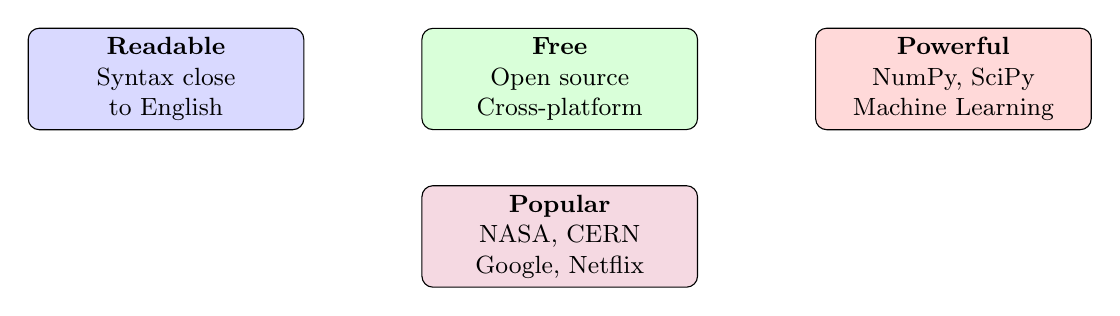
\begin{tikzpicture}[
  box/.style={rectangle, draw, fill=#1!15, rounded corners,
    minimum width=3.5cm, minimum height=0.8cm, align=center, font=\small}
]
\node[box=blue] at (0,0) {\textbf{Readable}\\Syntax close\\to English};
\node[box=green] at (5,0) {\textbf{Free}\\Open source\\Cross-platform};
\node[box=red] at (10,0) {\textbf{Powerful}\\NumPy, SciPy\\Machine Learning};
\node[box=purple] at (5,-2) {\textbf{Popular}\\NASA, CERN\\Google, Netflix};
\end{tikzpicture}
\end{center}

\section{Your First Program}

\begin{codeblock}[title=\textbf{Python}]
\begin{minted}{python}
print("Hello, future scientist!")
\end{minted}
\end{codeblock}

\begin{codeoutput}
\begin{verbatim}
Hello, future scientist!
\end{verbatim}
\end{codeoutput}

Congratulations! You just wrote your first program. The \py{print()}\index{print} function displays text on screen.

\section{Python as a Calculator}

Python can perform all basic mathematical operations:

\begin{codeblock}[title=\textbf{Python --- Basic calculations}]
\begin{minted}{python}
# Addition and subtraction
print(3 + 5)
print(10 - 4)

# Multiplication and division
print(6 * 7)
print(15 / 4)     # Real division
print(15 // 4)    # Integer division
print(15 % 4)     # Remainder (modulo)

# Exponentiation
print(2 ** 10)     # 2 to the power 10
\end{minted}
\end{codeblock}

\begin{codeoutput}
\begin{verbatim}
8
6
42
3.75
3
3
1024
\end{verbatim}
\end{codeoutput}

\begin{keyformulas}[title=\textbf{Arithmetic Operators}]
\begin{tabular}{lll}
\toprule
\textbf{Operator} & \textbf{Meaning} & \textbf{Example} \\
\midrule
\py{+} & Addition & \py{3 + 5} $= 8$ \\
\py{-} & Subtraction & \py{10 - 4} $= 6$ \\
\py{*} & Multiplication & \py{6 * 7} $= 42$ \\
\py{/} & Real division & \py{15 / 4} $= 3.75$ \\
\py{//} & Integer division & \py{15 // 4} $= 3$ \\
\py{\%} & Modulo (remainder) & \py{15 \% 4} $= 3$ \\
\py{**} & Exponentiation & \py{2 ** 10} $= 1024$ \\
\bottomrule
\end{tabular}
\end{keyformulas}

\section{Comments}

\textbf{Comments}\index{comment} are notes for humans. Python ignores them completely.

\begin{codeblock}[title=\textbf{Python}]
\begin{minted}{python}
# This is a comment — Python ignores it
print(2 + 3)   # You can comment at end of line

# Speed of light in m/s
c = 299792458
print(f"Speed of light: {c} m/s")
\end{minted}
\end{codeblock}

\begin{codeoutput}
\begin{verbatim}
5
Speed of light: 299792458 m/s
\end{verbatim}
\end{codeoutput}

\begin{bestpractice}
Comment your code to explain \textbf{why} you are doing something, not \textbf{what} you are doing. A good comment says ``Speed of light in m/s'', not ``Assign 299792458 to c''.
\end{bestpractice}

\section{Scientific Example: Kinetic Energy}

Let us compute the kinetic energy $E_k = \frac{1}{2}mv^2$ of an object:

\begin{codeblock}[title=\textbf{Python --- Kinetic energy}]
\begin{minted}{python}
# Data
mass = 75.0        # kg (a person)
velocity = 10.0    # m/s (fast running)

# Compute kinetic energy
Ek = 0.5 * mass * velocity ** 2

print(f"Mass     : {mass} kg")
print(f"Velocity : {velocity} m/s")
print(f"Energy   : {Ek} J")
\end{minted}
\end{codeblock}

\begin{codeoutput}
\begin{verbatim}
Mass     : 75.0 kg
Velocity : 10.0 m/s
Energy   : 3750.0 J
\end{verbatim}
\end{codeoutput}

\section{Errors: Don't Be Afraid!}

\begin{errmark}
Errors are \textbf{normal} and part of learning. Python helps by indicating the error type and line number.

\begin{codeblock}[title=\textbf{Python --- Common errors}]
\begin{minted}{python}
# Syntax error: missing parenthesis
# print("Hello"
# SyntaxError: '(' was never closed

# Name error: undefined variable
# print(x)
# NameError: name 'x' is not defined

# Type error: impossible operation
# "abc" + 5
# TypeError: can only concatenate str to str

# Division by zero
# 10 / 0
# ZeroDivisionError: division by zero
\end{minted}
\end{codeblock}

\textbf{Golden rule}: always read the error message \textbf{from bottom to top}. The last line tells you what went wrong.
\end{errmark}

\section{Interactive Mode vs Scripts}

\begin{center}
\begin{tikzpicture}[
  box/.style={rectangle, draw, fill=#1!15, rounded corners,
    minimum width=5cm, minimum height=2cm, align=center, font=\small}
]
\node[box=blue] (inter) at (0,0) {\textbf{Interactive mode}\\(Jupyter, console)\\Test, explore\\Immediate feedback};
\node[box=green] (script) at (7,0) {\textbf{Script}\\(.py file)\\Complete program\\Reusable};
\draw[-{Stealth},thick,dashed] (inter) -- node[above,font=\scriptsize]{Prototype} node[below,font=\scriptsize]{then automate} (script);
\end{tikzpicture}
\end{center}

\section{Mini-Project: Unit Conversions}

\begin{projet}
Write a program that converts temperatures between Celsius and Fahrenheit.

\textbf{Formulas}: $F = \frac{9}{5}C + 32$ and $C = \frac{5}{9}(F - 32)$

\begin{codeblock}[title=\textbf{Python --- Converter}]
\begin{minted}{python}
# Celsius -> Fahrenheit
celsius = 100
fahrenheit = (9/5) * celsius + 32
print(f"{celsius}°C = {fahrenheit}°F")

# Fahrenheit -> Celsius
fahrenheit = 72
celsius = (5/9) * (fahrenheit - 32)
print(f"{fahrenheit}°F = {celsius:.1f}°C")

# Conversion table
print("\n--- Conversion Table ---")
print(f"{'°C':>6}  {'°F':>6}")
for c in range(0, 101, 10):
    f = (9/5) * c + 32
    print(f"{c:>6}  {f:>6.1f}")
\end{minted}
\end{codeblock}

\begin{codeoutput}
\begin{verbatim}
100°C = 212.0°F
72°F = 22.2°C

--- Conversion Table ---
    °C      °F
     0    32.0
    10    50.0
    20    68.0
    30    86.0
    40   104.0
    50   122.0
    60   140.0
    70   158.0
    80   176.0
    90   194.0
   100   212.0
\end{verbatim}
\end{codeoutput}
\end{projet}

\section{Exercises}

\begin{exercise}[$\star$ --- Guided]
Compute the area of a circle with radius $r = 5$ using $A = \pi r^2$. Use \py{3.14159} for $\pi$.
\end{exercise}

\begin{exercise}[$\star$ --- Guided]
Compute the distance between points $(x_1, y_1) = (1, 2)$ and $(x_2, y_2) = (4, 6)$ using $d = \sqrt{(x_2-x_1)^2 + (y_2-y_1)^2}$. Hint: $\sqrt{x} = x^{0.5}$.
\end{exercise}

\begin{exercise}[$\star\star$ --- Independent]
Newton's law of gravitation gives the force between two masses: $F = G\frac{m_1 m_2}{r^2}$, with $G = 6.674 \times 10^{-11}$~N$\cdot$m$^2$/kg$^2$. Compute the force between Earth ($m_1 = 5.972 \times 10^{24}$~kg) and Moon ($m_2 = 7.342 \times 10^{22}$~kg), separated by $r = 3.844 \times 10^{8}$~m.
\end{exercise}

\begin{exercise}[$\star\star\star$ --- Scientific Challenge]
Compute the de Broglie wavelength $\lambda = h / (mv)$ for an electron ($m = 9.109 \times 10^{-31}$~kg) moving at $v = 10^6$~m/s, with $h = 6.626 \times 10^{-34}$~J$\cdot$s. Compare with the size of an atom ($\sim 10^{-10}$~m).
\end{exercise}

\begin{keyformulas}[title=\textbf{Chapter Summary}]
\begin{itemize}
\item \py{print()} displays text and values.
\item Python knows: \py{+}, \py{-}, \py{*}, \py{/}, \py{//}, \py{\%}, \py{**}.
\item Comments start with \py{#}.
\item Errors are normal --- read the message from bottom to top.
\item A \py{.py} script is a reusable program.
\end{itemize}
\end{keyformulas}
